\documentclass{scrreprt}

\usepackage[utf8]{inputenc}
\usepackage{graphicx}
\usepackage[french]{babel}
\usepackage{multirow}
\usepackage[dvipsnames]{xcolor}
\usepackage[allbordercolors=white]{hyperref}
\usepackage{mdframed}
\usepackage{pgfplotstable}
\usepackage{tikz-3dplot}
\usepackage[OT1]{fontenc}
\usepackage{minted}
\usepackage{caption}
\usepackage[bottom=2cm,footskip=8mm]{geometry}

\newmdenv[
rightline=false,
topline=false,
bottomline=false,
backgroundcolor=BurntOrange!5,
fontcolor=BrickRed,
linecolor=Red,
linewidth=1pt]{problem}


\newmdenv[
rightline=false,
topline=false,
bottomline=false,
backgroundcolor=ForestGreen!5,
fontcolor=OliveGreen,
linecolor=Green,
linewidth=1pt]{result}


\newmdenv[
rightline=false,
topline=false,
bottomline=false,
backgroundcolor=Cyan!5,
fontcolor=Blue,
linecolor=NavyBlue,
linewidth=1pt]{info}

%Page style

\pagestyle{headings}
\pagenumbering{arabic}
\KOMAoption{headsepline}{true}
\KOMAoption{footsepline}{true}
\KOMAoption{twoside}{false}
\KOMAoption{abstract}{false}
\KOMAoption{DIV}{10}


%Title page


\titlehead{\centering {\Large \bfseries RAPPORT DE PROJET}\\
	\itshape{ 2ème année de licence d'informatique}}
\subject{}
\title{\Huge \bfseries INTERPRETATION DE LANGUAGE VIA FACTORIO}
\author{Réalisé par \\Christopher JACQUIOT}
\date{}
\publishers{
\includegraphics[width=0.5\textwidth]{pics/factorio-logo.png}\\
	\vspace{20px}
	
\includegraphics[width=0.5\textwidth]{pics/logo_long.png}}

\makeglossary

\begin{document}
	
	\setminted[hs]{
		breaklines,
		mathescape,
		linenos,
		numbersep=5pt,
		frame=leftline,
		numbersep=5pt,
		xleftmargin=0pt,
	}
	
	
	\maketitle
	\pagenumbering{roman}
	
	\tableofcontents
	\listoffigures
	\listoftables
	\chapter*{Remerciements}
	\paragraph{} 
	Je tiens à remercier mon professeur M. François RIOULT pour ce sujet de projet et sa supervision attentive.
	
	
	Nous remercions l'équipe de Factorio pour leur investissement zélé dans le développement, l'optimisation et le polissage de leur jeu.
	Nous remercions également le joueur DemiPixel pour sa librairie de manipulation de blueprints très pratique.
	
	\pagenumbering{arabic}
	
	\chapter{Introduction}
	
	\section{Pourquoi utiliser Factorio?}
	
	\subsection{Qu'est-ce-que Factorio?} 
	
	\paragraph{}
	
	\textbf{Factorio} un jeu de logistique, stratégie, résolution de problèmes et de gestion de ressources fortement inspiré des packs de mods \textbf{Feed The Beast (FTB)} pour le jeu \textbf{Minecraft}, où le joueur doit automatiser la production et la transformation de ressources afin de pouvoir progresser dans le jeu par le biais de tapis roulants, de trains, de logique et de machines.
	
	\begin{figure}[h]
		\centering
		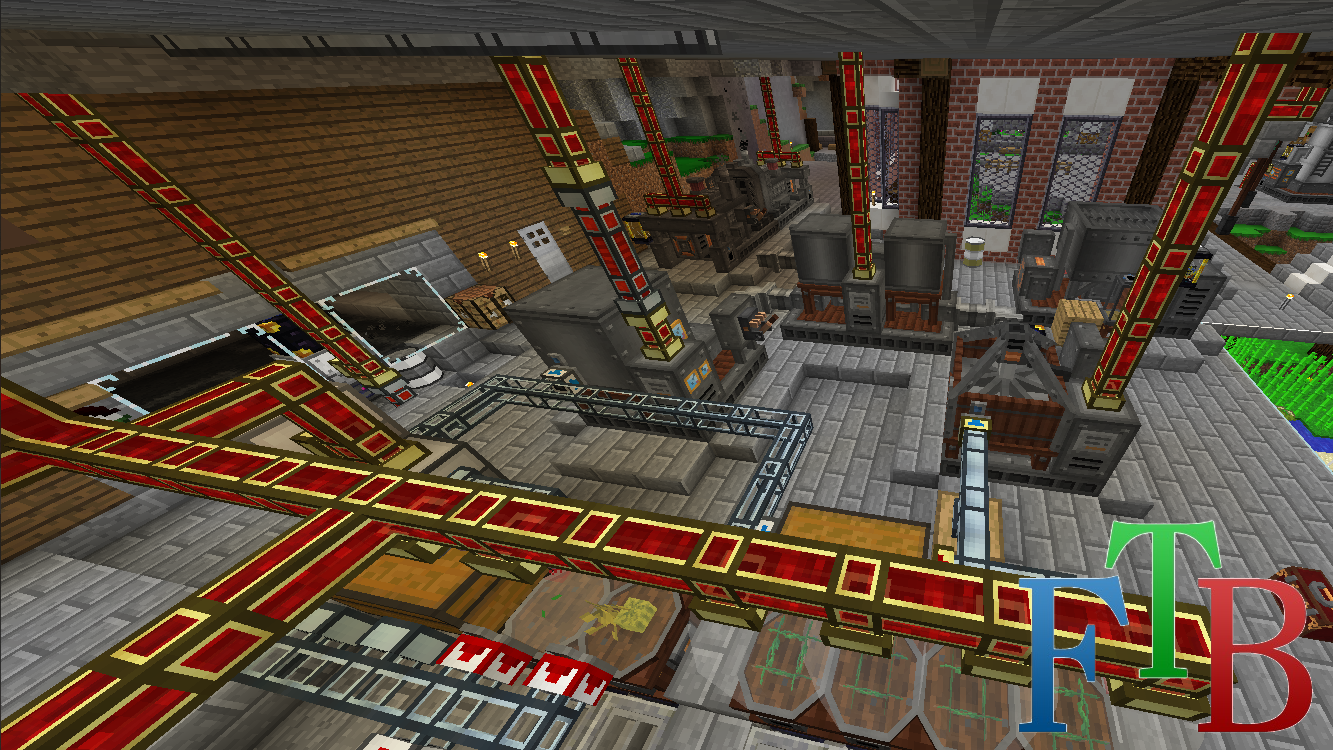
\includegraphics[width=0.8\linewidth]{pics/ftb-presentation.png}
		
		\caption{Exemple d'automatisation Feed The Beast}
	\end{figure}
	
	\begin{figure}[h]
		\centering
		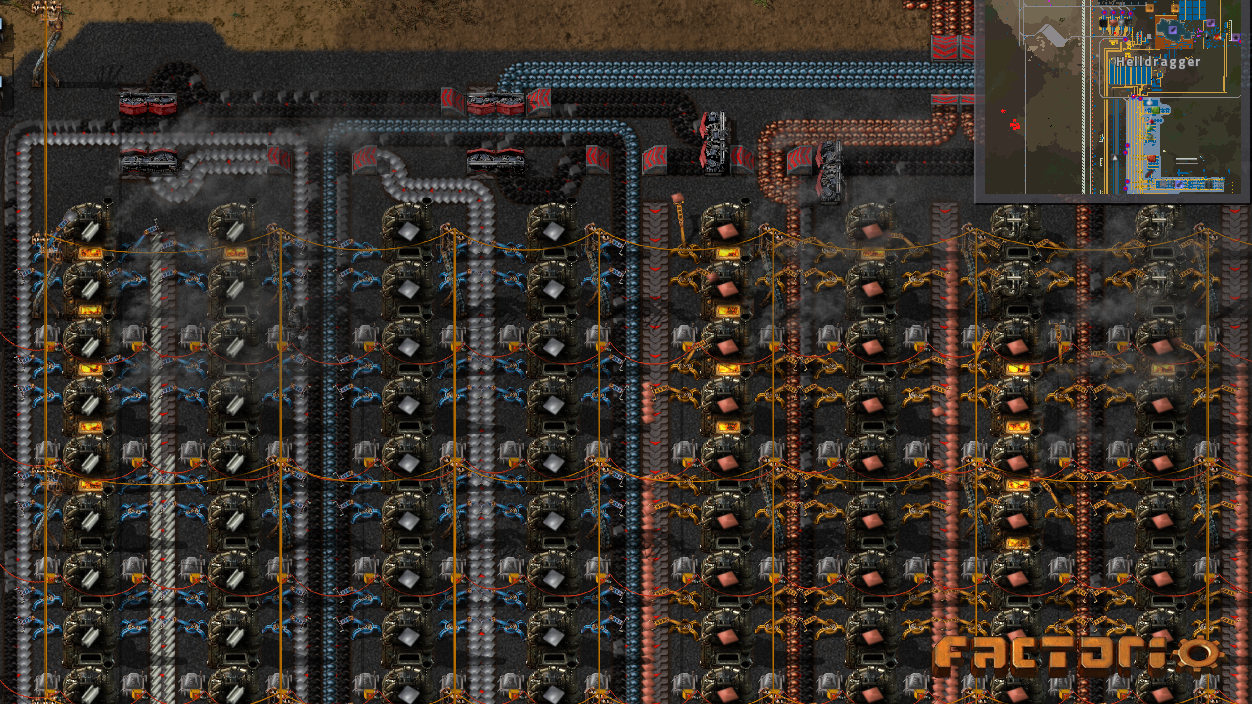
\includegraphics[width=0.8\linewidth]{pics/factorio-presentation.png}
		
		\caption{Exemple d'automatisation Factorio}
	\end{figure}
	
	
	Ce jeu en particulier présente au joueur la mécanique de jeu du réseau logique qui permet à chaque itération du moteur de jeu de transmettre des signaux spécifiques pouvant avoir pour toute valeur entière signée sur 32 bits.
	À cela s'ajoute la présence de méthodes d'utilisation et d'évaluations de ces signaux qui permettent de réaliser des systèmes d'automatisation logique et complexes, notamment les combinateurs arithmétiques et combinateurs logiques que nous allons voir plus en détails plus bas.
	
	
	\begin{figure}[h]
		\centering
		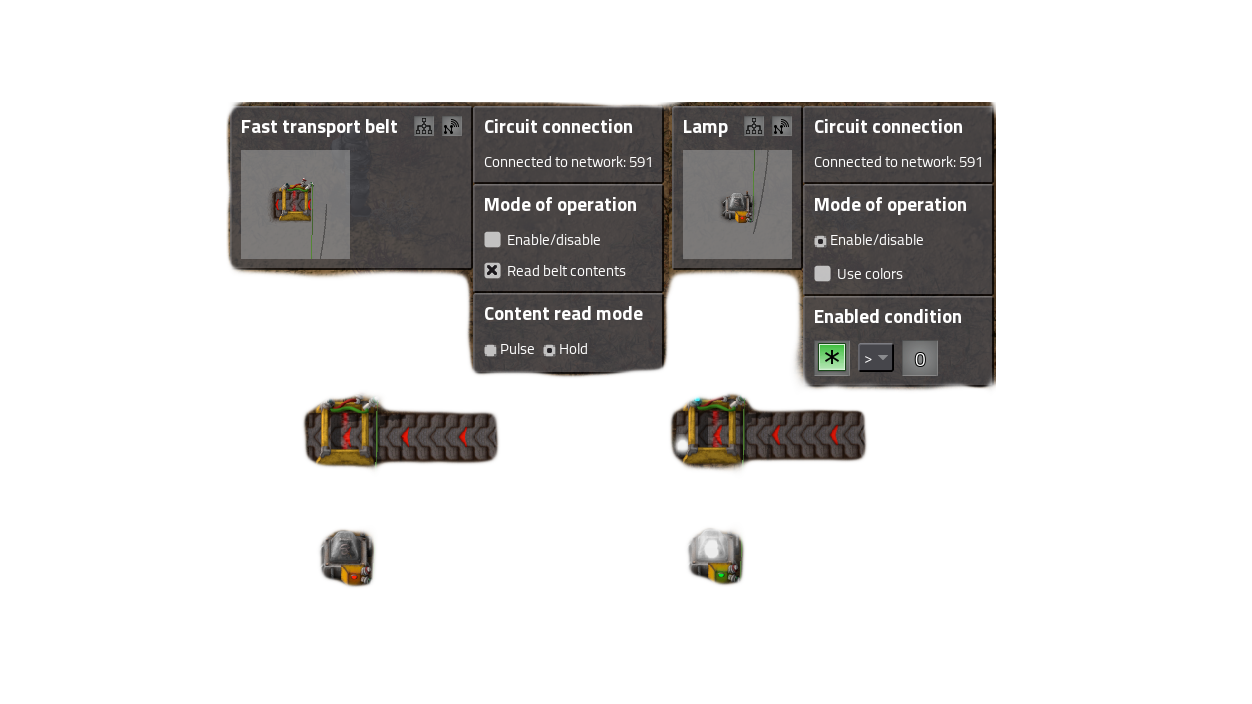
\includegraphics[width=0.8\linewidth]{pics/factorio-logic-basis.png}
		
		\captionof{figure}{Exemple de logique  basique: Détecteur d'objet}
	\end{figure}
	
	Le jeu lui même intègre aussi un système de \textbf{blueprint}, des plans de constructions récupérable et partageable hors du jeu permettant de construire divers systèmes complexes entre joueurs.
	
	
	\subsection{Les circuits logiques}
	
	\paragraph{Les réseaux logiques} 
	sont construits en utilisant des câbles rouge ou vert, et permettent le contrôle de récepteurs, basé sur les informations envoyées sur le réseau par les émetteurs connectés. 
	La plupart des émetteurs sont des périphériques de stockage, et émettent les informations de leur contenu sur des signaux spécifiques, basés sur le type des objets ou fluides que le périphérique de stockage contient. 
	
	Chaque réseau logique contient un signal pour chaque type d'objet du jeu, ainsi que 45 signaux virtuels supplémentaires qui agissent en tant que signaux définis par le joueur. 
	Les signaux spéciaux ['Tout'], ['N'importe quoi'] et ['Chacun'] sont aussi disponibles.
	
	
	
	
	\subsection{Le combinateur arithmétique}
	
	\begin{minipage}[t]{\textwidth}
		
		{
			\centering
			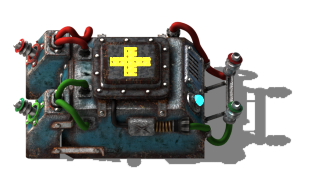
\includegraphics{pics/factorio-arithmetic.png}
			\captionof{figure}{Combinateur arithmétique}
		}
		
		
	\end{minipage} 
	
	
	\paragraph{}
	Le combinateur arithmétique évalue des opérations arithmétiques à partir de ses signaux d'entrée et émet le résultat sur les signaux spécifiés dans l'emplacement de signal de sortie. 
	L'entrée et la sortie peut se faire sur n'importe quel signal d'objet ou signal virtuel.
	
	\paragraph{Branchements} 
	Le combinateur arithmétique se connecte à un réseau rouge ou vert sur son coté \textbf{entrée} représenté par les terminaux font partie intégrante du combinateur et ressemblent a des branchements ampoules, et réalise une opération arithmétique qui sera émise à partir du coté \textbf{sortie} d'où les câbles de sortie semblent sortir un peu du combinateur. 
	
	\paragraph{Retour de signal}
	Notez que le réseau d'entrée et le réseau de sortie \textbf{ne sont pas le même réseau}.
	Connecter le réseau de sortie au réseau d'entrée résultera en une boucle de retour. 
	
	Par exemple, ajouter 1 à la valeur des plaques de cuivre et l'émettre en tant que plaques de cuivre est une action qui résultera en une boucle infinie si la sortie est connectée à l'entrée. 
	La valeur des plaques de cuivre va alors vite (mais pas instantanément) augmenter. 
	La vitesse à laquelle celle ci augmente est de 1 par mise à jour du moteur de jeu, autrement appelé \textbf{tick de jeu}. 
	
	Cette technique peut être combinée avec la logique de combinateur logique pour réaliser des horloges électroniques, des portes, et d'autres systèmes;
	
	\paragraph{Signal ['Chacun']}
	Ce combinateur peut utiliser le signal ['Chacun'] à la fois en entrée et en sortie, auquel cas tous les signaux différents de zéro vont se voir calculés séparément selon l'opération du combinateur et leur résultat émis sur le coté sortie.
	Avoir le signal ['Chacun'] à la fois en entrée et en sortie et utiliser une opération non modifiante (comme ajouter 0) est équivalent à un câble à sens unique; toutes les informations du réseau d'entrée est copiée au réseau de sortie, mais l'inverse n'est pas vrai.
	
	\paragraph{Jonction de réseaux}
	Les combinateurs arithmétiques peuvent être utilisés pour joindre deux réseaux sur leur coté entrée et renvoyer la somme de leurs réseaux.
	
	\subsection{Le combinateur logique}
	\begin{minipage}[t]{\textwidth}
		
		{
			\centering
			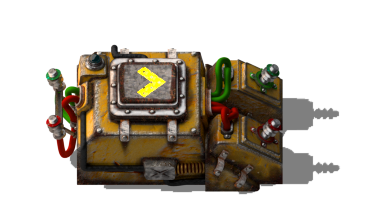
\includegraphics{pics/factorio-decider.png}
			\captionof{figure}{Combinateur logique}
		}
		
	\end{minipage} 
	
	\paragraph{}
	Le combinateur logique fonctionne comme un combinateur arithmetique, mais est designé pour comparer des valeurs.
	Essentiellement, c'est un conditionnel.
	
	En termes de connexion, retour, et de signaux, il fonctionne tel que décris plus haut. De plus, il peut gérer les signaux ['Tout'] et ['N'importe quoi'], et permet de réaliser des comparaisons logiques. 
	
	\subsection{L'émetteur de constante}
	\begin{minipage}[t]{\textwidth}
		
		
		{
			\centering
			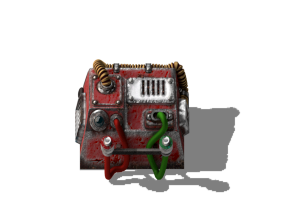
\includegraphics{pics/factorio-constant.png}
			\captionof{figure}{Émetteur de constante}
		}
		
	\end{minipage}
	
	\paragraph{}
	L'émetteur de constante émet jusqu'à 15 valeurs sur n'importe quel signal sur tous les réseaux logiques qui y sont branchés. 
	(Vous ne pouvez pas spécifier si une valeur devrait être envoyé sur le réseau rouge ou vert uniquement; si vous avez besoin de deux valeurs différentes, utilisez deux émetteurs, un pour chaque couleur de cable.) 
	Vous pouvez utiliser n'importe quel signal d'objet ou n'importe quel signal virtuel.
	
	\begin{info}
		Notez qu'utiliser deux emplacements de signaux pour émettre des valeurs sur le même signal reviens à émettre la somme des deux valeurs sur un seul emplacement.
	\end{info}
	
	\section{Présentation du projet}
	
	\paragraph{Quel est ce projet?}
	
	La gestion de la logique de factorio et ses nombreuses applications en jeu permettent d'avoir un rendu particulièrement visuel et intuitif des applications de la logique en jeu.
	Pouvoir activer des machines ou des routes selon certaines conditions permet en effet de visualiser facilement le resultat de l evaluation d un signal logique.
	
	\begin{problem}
		Pouvons-nous interprêter un langage par le biais de ce systême logique et faire réagir un système en conséquence?
	\end{problem}
	
	Les blueprints de Factorio étant aussi juste des fichiers de données encodés en base64 pour un transfert plus aisé entre joueurs et factorio, il est donc possible de manipuler ces blueprints pour en générer de plus grand et plus complexes par programmation.
	
	Nous avons pour cela la librairie node.js factorio- blueprint créée par le moddeur Demipixel, qui permet de manipuler aisément des blueprints.
	Grâce à cela nous pouvons faire un lien entre du code écrit sur fichier texte et des systèmes copiable/collable dans factorio:
	
	
	\begin{problem}
		Pouvons nous donc interprêter n'importe quel language écrit dans un fichier sur factorio?
	\end{problem}
	
	\section{Le language}
	
	\paragraph{Qu'es ce qu'un language?}
	Un langage est un ensemble de mots ayant un sens défini dans un certain contexte.
	Dans notre cas, le language as pour but de représenter notre language mathématique habituel ainsi que des opérations de stockage: Nous voulons pouvoir manipuler des valeurs et les retrouver ou les sauvegarder pour plus tard.
	
	Nous voulons aussi pouvoir determiner des branches conditionnelles, pour determiner une séquence d'instructions à suivre selon des conditions particulières.
	
	\paragraph{Qu'es ce qu'un mot?}
	Dans notre cas nos mots seront différenciés par un nombre différent, sur le signal E.
	Ainsi par exemple, le mot de l'instruction LOAD ADDR CONTENT INTO REGISTER A sera la valeur 1 sur le signal E, ou le mot de  l'instruction NOT REGISTER A INTO A sera la valeur 16 sur ce meme signal.
	
	\begin{info}
		La liste détaillée de toutes les instructions disponibles est trouvable en annexes.
	\end{info}
	
	\paragraph{Qu'es ce qu'une instruction?}
	Nos instructions sont simplement la combinaison d'un mot d'instruction sur le signal E et d' arguments sur les signaux 1, 2 etc.. selon les instructions.
	
	\begin{figure}[h]
		\centering
		\includegraphics[width=0.8\linewidth,draft]{pics/factorio-instruction.png}
		
		\caption{Exemple d'instruction}
	\end{figure}
	
	
	
	Ces instructions vont être décodées et interprêtées par un processeur d'instructions, qui va gêrer la synchronisation des étapes entre recupération des instructions, leur décodage et l'exécution. 
	
	\section{Le processeur d'instructions}
	
	
	
	\paragraph{Une histoire de contexte}
	Afin de pouvoir analyser et synchroniser nos opérations, nous allons avoir besoin de stocker en mémoire l'instruction actuelle afin de pouvoir accèder à son code ou ses arguments en temps voulu.
	
	Pour cela nous allons avoir besoin d'un registre mémoire d'instruction!
	Qui contiendra notre instruction actuelle et ses arguments.
	\begin{figure}[h]
		\centering
		\includegraphics[width=0.8\linewidth,draft]{pics/factorio-diag-regINSTR.png}
		
		\caption{Diagramme d'utilisation d'une mémoire d'instruction}
	\end{figure}
	
	Afin de pouvoir savoir où chercher la prochaine instruction, nous allons aussi avoir besoin d'une adresse modifiable, vers laquelle nous diriger à chaque cycle d'instruction.
	
	Pour cela nous allons avoir besoin d'un autre registre mémoire nommé compteur de programme!
	Cela reste basiquement un compteur qui sera incrémenté à chaque nouveau cycle ou sera modifié selon le résultat d'une fonction conditionnelle par exemple.
	
	
	\begin{figure}[h]
		\centering
		\includegraphics[width=0.8\linewidth,draft]{pics/factorio-diag-regPC.png}
		
		\caption{Diagramme d'utilisation d'un compteur de programme}
	\end{figure}
	
	\paragraph{Un ballet synchronisé de micro-opérations}
	Avant de pouvoir manipuler des données ou donner des instructions entre différents composants, nous allons devoir synchroniser les lectures et écritures des différentes cellules mémoires de notre machine, que ce soit entre registre ou entre cpu et memoire.
	Pour cela nous allons avoir besoin de \textbf{micro-instructions} dédiées aux opérations les plus délicates et réservées au processeur, qui seront appelées pour certaines simultanément. 
	
	\begin{info}
		La liste complète de ces micro-instructions et le micro-code utilisé est disponible dans leurs propre sections respectives en annexes.
	\end{info}
	
	Par exemple, afin de pouvoir créer une opération simple telle que LOAD-A, nous allons devoir réaliser la séquence de micro-instructions simultanées suivante: 
	
	\begin{minted}{hs}
WIRE regINSTR regMAR; READ regINSTR; WRITE regMAR; -- write address from regINSTR to regMAR
WIRE mem regA; READ mem; WRITE regA; -- write data from mem to regA
	\end{minted}
	
	
	Nous allons donc avoir besoin d'un lecteur de micro-code basique afin de pouvoir éxecuter ces diverses micro-instructions selon un timing et un ordre précis pour pouvoir créer des opérations de plus haut niveau et préparer notre cycle de récupération-décodage-éxecution d'instructions, le tout restant facile à modifier et à agrandir!
	
	\section{La manipulation de données}
	
	\paragraph{Une mémoire de travail!}
	Quand l'on doit travailler sur une valeur particulière, il peut être utile de s'en souvenir le temps de la modifier, plutôt que d'aller stocker puis re-récuperer le résultat à chaque nouvelle opération sur cette valeur.
	Les temps d'accès et d'écriture mémoire sont aussi significatifs, raison de plus donc pour les diminuer un maximum.
	
	\begin{figure}[h]
		\centering
		\includegraphics[width=0.8\linewidth,draft]{pics/factorio-diag-regA.png}
		
		\caption{Diagramme d'utilisation d'une mémoire de travail}
	\end{figure}
	
	Nous allons donc avoir besoin d'une simple mémoire de travail, capable de contenir une valeur basique et qui se mets à jour avec le résultat des opérations sur cette valeur!
	
	
	Ceci dis, il peut nous arriver de vouloir travailler sur de multiples valeurs à la fois, via des vecteurs.
	Afin de pallier au souci de devoir faire les operations une par une, nous pouvons paralléliser les choses! 
	Pour cela nous aurons besoin d un mode de calcul vectoriel, et comme pour les calculs sur valeur simple, il nous faut aussi une mémoire de travail pour cela: un registre vectoriel!
	
	\begin{figure}[h]
		\centering
		\includegraphics[width=0.8\linewidth,draft]{pics/factorio-diag-regV.png}
		
		\caption{Diagramme d'utilisation d'une mémoire de travail vectorielle}
	\end{figure}
	
	Si en revanche nous devons travailler sur un vecteur de valeurs, nous allons avoir besoin de pouvoir selectionner sur quelles valeurs travailler en plus des valeurs elles memes, pour eviter des problemes de calculs indéterminés.
	Les opérations sur le registre vectoriel ne devront alors se faire que sur les signaux acceptés par un masque vectoriel de booléen.
	
	
	\begin{figure}[h]
		\centering
		\includegraphics[width=0.8\linewidth,draft]{pics/factorio-diag-regVmask.png}
		
		\caption{Diagramme d'utilisation du masque vectoriel}
	\end{figure}
	
	\paragraph{Des opérations mathématiques!}
	Afin de pouvoir manipuler nos données stockées nous allons avoir besoin de regrouper et intégrer à notre système un maximum d'opérations mathématiques sur nos registres de travail.
	Pour le calcul sur valeur unique, nous allons pouvoir utiliser ce que l'on appelle communément une \textbf{Unité Arithmétique et Logique} traduit Arithmetic and Logic Unit (\textbf{ALU}).
	
	Ces unités permettent de sélectionner une opération particulière à partir d'un signal de commande et qui prends deux autres signaux en entrées, pour ressortir la valeur du résultat de cette opération.
	Ici le résultat est censé être stocké directement dans le registre A suite à la réalisation du calcul, qui sers de première entrée aux calculs.
	
	\begin{figure}[h]
		\centering
		\includegraphics[width=0.8\linewidth,draft]{pics/factorio-diag-ALU.png}
		
		\caption{Diagramme d'utilisation d'une ALU}
	\end{figure}
	
	De même pour notre manipulation de vecteurs, nous allons avoir besoin d'une \textbf{Unité Arithmétique et Logique Vectorielle} traduit Vectorial Arithmetic and Logic Unit (\textbf{VALU}), qui reste une simple ALU mais parallélisée pour un nombre donné de signaux.
	Ici nous avons créé un VALU pouvant calculer autant de signaux qu'une cellule mémoire vectorielle peut théoriquement gérer. 
	
	
	
	
	\section{Analyse du problème}
	
	
	
	
	\paragraph{Interprêter n'importe quel language}
	Pour interprêter n 'importe quel language, nous avons besoin d'un interpréteur de langage, qui peut donc avoir accès à sa définition stockée quelque part. Nous allons avoir besoin de mémoire. 
	
	Nous allons aussi avoir besoin d'une façon de réaliser toutes les opérations arithmétiques et logiques que l'on pourrait interprêter avec n'importe quel langage. Nous allons avoir besoin d'une Unité Logique et Arithmétique (ALU).
	
	Nous allons aussi avoir besoin de savoir à quel endroit de notre définition de langage nous nous trouvons à chaque instant pour determiner du prochain endroit a évaluer. Nous allons avoir besoin d un compteur de programme.
	
	Enfin pour simplifier cela nous allons avoir besoin d un moyen de coordonner les operations logiques entre la memoire et nos autres elements d interprêteur et de gerer les instructions pointees par le compteur de programme. Nous allons avoir besoin d'un séquenceur d instructions.
	
	Autrement dit, avec notre liste d instructions en annexes et notre systeme ci present, nous devrions pouvoir lire, interpréter et évaluer les instructions de tout programme utilisant les opérations mathématiques et logiques de base implémentées par factorio. 
	
	\part{Micro contrôlleur - architecture}
	\chapter{Résumé}
	
	\paragraph{Une machine de Turing complète?}
	
	Afin de pouvoir éxecuter n'importe quel langage sur notre machine, nous devons créer une machine capable d'émuler n'importe quel langage. Autrement dit, de pouvoir lire le fonctionnement d'une machine et de l'interprèter afin de reproduire les mêmes résultats que si on l avait construite indépendamment.
	
	Une machine de Turing pouvant alors émuler toute autre machine de Turing est une machine de Turing dite complète.
	Et en créer une à partir de Factorio est l'objectif de ce projet.
	
	\section{En quelques nombres}
	% temps par micro instruction * micro instructions par cycle => nombre de cycles par secondes (Hz)
	% taille d'une cellule memoire * nb adresses en 32 bit => taille totale potentielle en memoire
	
	\section{Survol de l'organisation spatiale}
	
	\section{Résumé des composants}
	
	
	
	
	\chapter{Mémoire in-game}
	
	\paragraph{Précisions sur les pertes de courant}
	Sur Factorio, les pertes de courant ne font pas perdre les valeurs stockées dans les combinateurs, ainsi contrairement à la RAM habituelle qui perds ses données après une coupure électrique, la mémoire dans Factorio as de base un fonctionnement de mémoire non volatile, comme de la EEPROM ou de la mémoire Flash.
	
	\section{Cellule mémoire de base}
	% Registre 1ko
	
	\section{Registres basiques}
	% bus dédié
	
	\section{Mémoire à accès aléatoire - RAM}
	% bus mémoire et plage d'adresse partagée avec le bios en rom
	% adressage de chaque cellule par une addresse spécifique
	
	\section{Mémoire à lecture seule - ROM}
	% bus mémoire et plage d'adresse partagée avec la ram, contient l adresse 0 comme adresse de bootloading.
	% ecriture manuelle du contenu des lignes de code.
	
	\section{Registre d'adresse mémoire - MAR}
	% registre contenant la prochaine adresse mémoire visée
	
	\section{Registre de donnée mémoire - MDR}
	% registre contenant le contenu lu dans la dernière lecture mémoire
	% L autre sens pourrait aussi être obligé mais par soucis d'économies d'instructions, non.
	
	\chapter{Séquenceur d'instructions}
	
	\section{Registre program counter - PC}
	% Registre contenant la position actuelle dans le programme actuellement en train d etre lu.
	
	\section{Registre d'instruction - INSTR}
	% Registre qui contient l instruction pointée par le registre PC.
	
	\section{Cycle Récupération-Décodage-Éxecution}
	% Micro code qui gère le flow de notre microcontrolleur
	
	\section{Instructions internes et externes}
	% Differentiation micro instructions et instructions 
	
	\chapter{Gestion d'instructions}
	
	\section{Généralités}
	% Zones dediees
	% Activation selon le bus d instructions
	% Jouent le rôle de coordinateurs de commandes io specifiques
	
	\section{Lecture-Écriture}
	% Parlons du switch généralisé entre tous les bus différents
	% Avantage du bus dédié => on evite l étape de temporarisation des données entre la lecture et l ecriture entre deux espaces memoires differents.
	% Avantage d adressage direct => On evite le clusterfuck de cable lié à autant de bus différents et est plus générique.
	
	
	
	\chapter{Opérations arithmétiques}	
	
	\section{Registre arithmétique - A}
	% registre tampon et automatiquement mis a jour a chaque operation arithmetique.
	% un seul signal autorisé
	
	\section{Unité Arithmétique et Logique - ALU}
	% liste des opérations possibles
	% ordre des operateurs regA op MDR
	
	\chapter{Opérations vectorielles}
	
	\section{Registre vectoriel - VECT}
	% registre tampon et automatiquement mis à jour à chaque opération vectorielle
	% tous les 204? signaux d objets sont autorisés
	
	\section{Registre mask - MASK}
	% registre de masquage pour un contrôle plus fin des opérations vectorielles sur reg V
	
	\section{Unité Vectorielle Arithmétique et Logique - VALU}
	% Memes operations que le ALU
	% ordre des operateurs regVi = regVi op MDRi ssi regMaski == True
	
	
	\part{FactorioScript}
	
	\chapter{Présentation}
	\section{Le fond}
	% À quoi sert ce langage? 
	% Son objectif
	
	\section{La forme}
	% Comment il a été réalisé
	% Comment s'en servir basiquement
	
	\chapter{Syntaxe}
	% Les if, les boucles, les goto, etc...
	
	\chapter{Signification en jeu}
	% Ce que représente chacune des opérations possibles
	
	\part{Compilateur script vers Factorio}
	
	\chapter{Compilation ...}
	\section{... des instructions}
	% Procédé de compilation du langage en instructions spécifiques de la machine.
	
	\section{... du blueprint}
	%Procédé de compilation des instructions spécifiques vers le blueprint final.
	
	\chapter{Autres usages}
	\section{Compilation en logique séquentielle}
	% Parler de l'optique originale du langage
	% De pouvoir compiler des opérations sans avoir besoin de CPU pour les lire
	% En liant juste des combinateurs directement les uns apres les autres.
	
	\cleardoublepage
	\pagebreak
	\pagenumbering{Roman}
	\part{Annexes}
	
	
	\chapter{Instructions}
	\paragraph{This is what programs can use}
	Those instructions are the lowest level instructions programs can use to write their logic with. 
	They are defined in the microcode using sequences of micro- instructions, which can be seen in the next annexe.
	Those instructions are sole the content of a single compiled program memory cell.
	
	\textbf{$A$} refers to the content of the register A.
	
	\textbf{$PC$} refers to the content of the register PC.
	
	\textbf{$V$} refers to the content of the register V.
	
	\textbf{$V_{mask}$} refers to the content of the register MASK.
	
	\textbf{$MEM[1]$} refers to the memory cell content at the address contained in signal [1].
	
	The symbol $\vec{ }$ means the value will be considered as a vector.
	
	\paragraph{Unconditional jump}
	As an experimentation, a unconditional jump can be forced by using the signal $[J]$, containing the next instruction address. 
	
	\section{Memory}
	\begin{tabular}{l | l | l  l}
		[E] & NAME & ARGS [signal]:type & DESC \\
		01 & LOAD-A & [1]:address & $A = MEM[1]$\\
		02 & STORE-A & [1]:address & $MEM[1] = A$\\
		18 & LOAD-VEC & [1]:address & $\vec{V} = \vec{MEM[1]}$\\
		19 & LOAD-VMASK & [1]:address & $\vec{V_{mask}} = \vec{MEM[1]}$\\
		20 & STORE-VEC & [1]:address & $\vec{MEM[1]} = \vec{V}$\\
		21 & STORE-VMASK & [1]:address & $\vec{MEM[1]} = \vec{V_{mask}}$\\
	\end{tabular}
	
	\section{Jump and conditionals}
	\begin{tabular}{l | l | l  l}
		[E] & NAME & ARGS [signal]:type & DESC \\
		-- & JMP & [J]:address & PC = [J]\\
		03 & JMP-A-EQ & [1]:address, [2]:address & IF ($A = MEM[2]$): PC = [1]\\
		04 & JMP-A-LT & [1]:address, [2]:address & IF ($A < MEM[2]$): PC = [1]\\
		05 & JMP-A-LE & [1]:address, [2]:address & IF ($A \le MEM[2]$): PC = [1]\\
		06 & JMP-A-GT & [1]:address, [2]:address & IF ($A > MEM[2]$): PC = [1]\\
		07 & JMP-A-GE & [1]:address, [2]:address & IF ($A \ge MEM[2]$): PC = [1]\\
		08 & JMP-A-NE & [1]:address, [2]:address & IF ($A \ne MEM[2]$): PC = [1]\\
		10 & JMP-V-EQ & [1]:address & IF ($A = MEM[1]$): PC = A\\
		11 & JMP-V-LT & [1]:address & IF ($A < MEM[1]$): PC = A\\
		12 & JMP-V-LE & [1]:address & IF ($A \le MEM[1]$): PC = A\\
		13 & JMP-V-GT & [1]:address & IF ($A > MEM[1]$): PC = A\\
		14 & JMP-V-GE & [1]:address & IF ($A \ge MEM[1]$): PC = A\\
		15 & JMP-V-NE & [1]:address & IF ($A \ne MEM[1]$): PC = A\\
	\end{tabular}
	
	\section{Arithmetic}
	\begin{tabular}{l | l | l  l}
		[E] & NAME & ARGS [signal]:type & DESC \\
		09 & ARITHM & [1]:address, [2]:value=1 & $A = A \mathbf{*} MEM[1]$\\  
		09 & ARITHM & [1]:address, [2]:value=2 & $A = A \mathbf{/} MEM[1]$\\  
		09 & ARITHM & [1]:address, [2]:value=3 & $A = A \mathbf{+} MEM[1]$\\  
		09 & ARITHM & [1]:address, [2]:value=4 & $A = A \mathbf{-} MEM[1]$\\  
		09 & ARITHM & [1]:address, [2]:value=5 & $A = A \mathbf{\%} MEM[1]$\\  
		09 & ARITHM & [1]:address, [2]:value=6 & $A = A^{MEM[1]}$\\  
		09 & ARITHM & [1]:address, [2]:value=7 & $A = A \mathbf{<<} MEM[1]$\\  
		09 & ARITHM & [1]:address, [2]:value=8 & $A = A \mathbf{>>} MEM[1]$\\  
		09 & ARITHM & [1]:address, [2]:value=9 & $A = A \mathbf{\&} MEM[1]$\\  
		09 & ARITHM & [1]:address, [2]:value=10 & $A = A \mathbf{|} MEM[1]$\\  
		09 & ARITHM & [1]:address, [2]:value=11 & $A = A \mathbf{xor} MEM[1]$\\  
		16 & NOT-A & & $A = !A$\\ 
	\end{tabular}
	
	\section{Vectorial}
	\begin{tabular}{l | l | l  l}
		[E] & NAME & ARGS [signal]:type & DESC \\
		17 & VEC-VEC & [1]:address, [2]:value=1 & $\vec{V} = (\vec{V}\&\vec{V_{mask}}) \mathbf{*} \vec{MEM[1]}$\\  
		17 & VEC-VEC & [1]:address, [2]:value=2 & $\vec{V} = (\vec{V}\&\vec{V_{mask}}) \mathbf{/} \vec{MEM[1]}$\\  
		17 & VEC-VEC & [1]:address, [2]:value=3 & $\vec{V} = (\vec{V}\&\vec{V_{mask}}) \mathbf{+} \vec{MEM[1]}$\\  
		17 & VEC-VEC & [1]:address, [2]:value=4 & $\vec{V} = (\vec{V}\&\vec{V_{mask}}) \mathbf{-} \vec{MEM[1]}$\\  
		17 & VEC-VEC & [1]:address, [2]:value=5 & $\vec{V} = (\vec{V}\&\vec{V_{mask}}) \mathbf{\%} \vec{MEM[1]}$\\  
		17 & VEC-VEC & [1]:address, [2]:value=6 & $\vec{V} = (\vec{V}\&\vec{V_{mask}})^{\vec{MEM[1]}}$\\  
		17 & VEC-VEC & [1]:address, [2]:value=7 & $\vec{V} = (\vec{V}\&\vec{V_{mask}}) \mathbf{<<}\vec{MEM[1]}$\\  
		17 & VEC-VEC & [1]:address, [2]:value=8 & $\vec{V} = (\vec{V}\&\vec{V_{mask}}) \mathbf{>>}\vec{MEM[1]}$\\  
		17 & VEC-VEC & [1]:address, [2]:value=9 & $\vec{V} = (\vec{V}\&\vec{V_{mask}}) \mathbf{\&}\vec{MEM[1]}$\\  
		17 & VEC-VEC & [1]:address, [2]:value=10 &$\vec{V} = (\vec{V}\&\vec{V_{mask}}) \mathbf{|}\vec{MEM[1]}$\\  
		17 & VEC-VEC & [1]:address, [2]:value=11 & $\vec{V} = (\vec{V}\&\vec{V_{mask}})  \mathbf{xor}\vec{MEM[1]}$\\  
		22 & NOT-VEC & & $\vec{V} = !(\vec{V}\&\vec{V_{mask}})$\\ 
	\end{tabular}
	\chapter{Micro-instructions}
	
	
	
	\chapter{Micro-code}
	\chapter{Bootloader}
	
	\begin{thebibliography}{}
	\end{thebibliography}
	
	%% TEMPLATE pour chapitre
	
	%\chapter{PARTIE}
	
	%\section{Nécessités}
	
	%\paragraph{}
	
	%\section{Problème}
	
	%\paragraph{}
	
	%\begin{problem}
	
	%\end{problem}
	
	%\section{Approches possibles}
	
	%\paragraph{}
	
	%\section{Approche utilisée}
	
	%\paragraph{}
	
	%\begin{result}
	
	%\end{result}
	
	%\section{Remarques sur les résultats obtenus}
	
	%\paragraph{}
	
	%\section{Pistes d'amélioration}
	
	%\paragraph{}
	
	
\end{document}
